\section{Άσκηση 1}
\subsection{Πειραματική εκτίμηση των $k_m, k_T, k_0, k_μ, T_m$}

Στόχος της πρώτης εργαστηριακής άσκησης του ενισχυτικού εργαστηρίου είναι η μοντελοποίηση ενός συστήματος ηλεκτρικού κινητήρα. Τα μετρητικά συστήματα είναι μια ταχογεννήτρια για τη μέτρηση της ταχύτητας του άξονα και ένα ποτενσιόμετρο για τη μέτρηση της θέσης του άξονα. Το δομικό διάγραμμα του συστήματος ηλεκτρικός κινητήρας συνεχούς ρεύματος – ταχογεννήτρια δίνεται στο \Cref{blockdiagram}, όπου $U$ είναι η τάση εισόδου, $Ω$ η ταχύτητα περιστροφής της ταχογεννήτριας σε rpm, $Θ$ η θέση – τάση του άξονα του κινητήρα και $V_{tacho}$ η τάση στην ταχογεννήτρια.

\begin{figure}[H]
  \begin{center}
    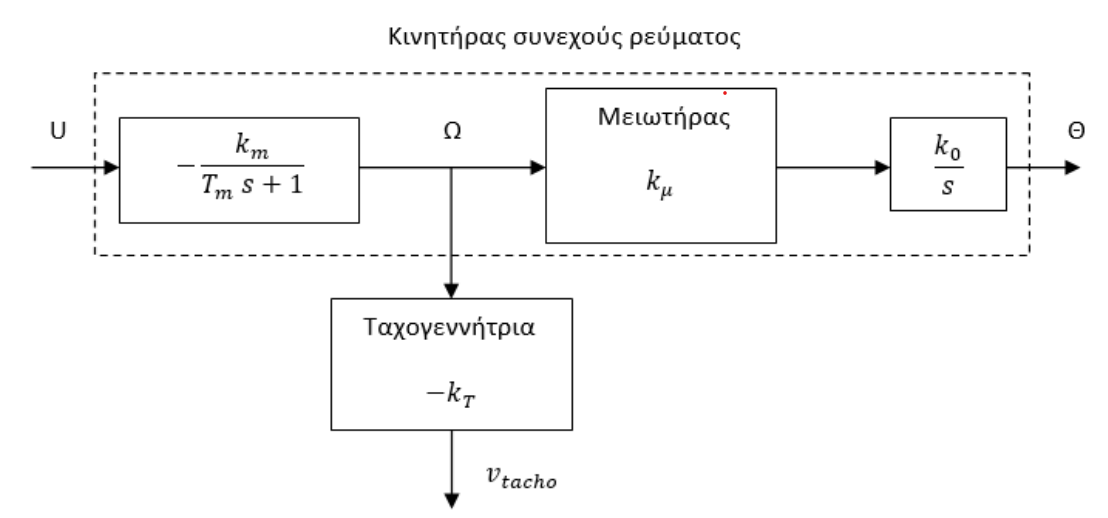
\includegraphics[width=\textwidth]{Images/blockdiagram.png}
  \end{center}
  \caption{Δομικό διάγραμμα συστήματος}
  \label{blockdiagram}
\end{figure}
Η μοντελοποίηση του συστήματος, λοιπόν, έγκειται στην εκτίμηση των παραμέτρων $k_m, k_T, k_0, k_μ, T_m$. Για αρχή, συνδέσαμε την έξοδο από το SW1 στο INPUT TO POWER AMPLIFIER και τα probes του παλμογράφου στο σημειο TACHO και στην έξοδο του SW1. Ανοίγοντας, τώρα, τον διακόπτη SW1, διεγήραμε το σύστημα με μία τάση εισόδου $10V DC$ και καταγράψαμε τα αποτελέσματα στον παλμογράφο για να δούμε το διάγραμμα της ταχύτητας. Από αυτό πήραμε τις μετρήσεις $V_{in} = 10V$ και $V_T = 2.78V$.

Από την συνάρτηση μεταφοράς $\dfrac{V_{tacho}}{U} = \dfrac{k_m k_T}{T_m s + 1}$ στην μόνιμη κατάσταση ($s=0$) παίρνουμε ότι 
\begin{equation}
	k_m k_T = \dfrac{V_T}{V_{in}} = 0.278
	\label{eq:kmkt}
\end{equation}
Για να υπολογίσουμε την παράμετρο $T_m$, βρήκαμε τη χρονική στιγμή κατα την οποία η απόκριση φτάνει στο 63,3\% της μέγιστης τιμής της, δηλαδή στην τιμή $V_m = V_T \cdot 63.3\% = 1.76V$ . Η οριζόντια απόσταση μεταξύ του άξονα y και του σημείου σταθεράς χρόνου είναι το $T_m$ το οποίο τελικά ισούται με $T_m = 0.47sec$.

Η παράμετρος $k_μ$ αντιστοιχεί στο λόγο της γωνίας στροφής του «άξονα εξόδου» προς τη γωνία στροφής του άξονα του κινητήρα. Γι' αυτό, στρέφοντας με το χέρι το δισκόφρενο που φέρει ο άξονας του κινητήρα για μία πλήρη στροφή, παρατηρήσαμε ότι ο «άξονας εξόδου» περιστρέφεται κατά $10$ μοίρες.\\ Άρα $k_μ = \dfrac{10}{360} = \dfrac{1}{36}$.

Επιλέγουμε μεταβλητές κατάστασης $x_1 = ω$ και $x_2 = θ$, τότε από το δομικό διάγραμμα παίρνουμε:
\begin{equation}
    \frac{Θ}{Ω} = k_μ \cdot \frac{k_0}{s} \Rightarrow \dot{x}_2 = k_μk_0x_1 \Rightarrow \frac{Δx_2}{Δt} = k_μk_0ω
    \label{eq1}
\end{equation}
Για να υπολογίσουμε το $\dfrac{Δx_2}{Δt}$ συνδέσαμε τον παλμογράφο στη θέση MOTOR POSITION INVERTED και πατώντας το HOLD μπορέσαμε να μετρήσουμε την κλίση της πριονωτής κυματομορφής που εμφανίζεται, καθώς και την
περίοδο $T_{\text{εξόδου}}$ μίας πλήρους περιστροφής του άξονα εξόδου. Λάβαμε τις μετρήσεις $\dfrac{Δx_2}{Δt} = \dfrac{11.3}{0.983} = 11.495$ και $T_{\text{εξόδου}} = 0.983sec$. 

Με μέθοδο των τριών μπορούμε να υπολογίσουμε το $ω_{\text{εξόδου}} = \dfrac{60}{T_{\text{εξόδου}}} = \dfrac{60}{0.983} = 61.037$. Οι στροφές, όμως, στην έξοδο είναι μειωμένες κατά $\dfrac{1}{k_μ} = 36$, άρα $ω = 36 \cdot ω_{\text{εξόδου}} = 36 \cdot 61.04 = 2197.33$rpm

Οπότε από την \Cref{eq1} έχουμε τελικά $k_0 = \dfrac{Δx_2}{Δt k_μ ω} = \dfrac{11.3 \cdot 36}{0.983 \cdot 2197.33} = 0.188$

Τέλος, έχουμε ότι $V_T = k_T ω \Rightarrow k_T = \dfrac{V_T}{ω} = \dfrac{2.78}{2197.33} = 1.27 \cdot 10^{-3}$

Και απο την \Cref{eq:kmkt} βρίσκουμε ότι $k_m = \dfrac{0.278}{k_T} = \dfrac{0.278}{1.27 \cdot 10^{-3}} = 218.89$

Συνοπτικά, η πειραματική εκτίμηση των ζητούμενων παραμέτρων είναι η εξής:

\begin{align*}
    k_m &= 218.89 \\
    k_T &= 1.27 \cdot 10^{-3} \\
    k_0 &= 0.188 \\
    k_μ &= \frac{1}{36} \\
    T_m &= 0.47sec
\end{align*}